\documentclass[journal]{IEEEtran}

\usepackage[pdfpagemode={UseOutlines},bookmarks=true,bookmarksopen=true,
   bookmarksopenlevel=0,bookmarksnumbered=true,hypertexnames=false,
   colorlinks,linkcolor={blue},citecolor={blue},urlcolor={blue},
   pdfstartview={FitV},unicode,breaklinks=true]{hyperref}

% *** MATH PACKAGES ***
\usepackage{amsmath,amssymb}

% *** GRAPHICS RELATED PACKAGES ***
\ifCLASSINFOpdf
	\usepackage[pdftex]{graphicx}
	\graphicspath{{images/}}
	% \DeclareGraphicsExtensions{.pdf,.jpeg,.png}
\else
	\usepackage[dvips]{graphicx}
	\graphicspath{{images/}}
	% \DeclareGraphicsExtensions{.eps}
\fi

% *** SUBFIGURE PACKAGES ***
\ifCLASSOPTIONcompsoc
  \usepackage[caption=false,font=normalsize,labelfont=sf,textfont=sf]{subfig}
\else
  \usepackage[caption=false,font=footnotesize]{subfig}
\fi

\usepackage{listings,color}

\definecolor{dkgreen}{rgb}{0,0.6,0}
\definecolor{gray}{rgb}{0.5,0.5,0.5}
\definecolor{mauve}{rgb}{0.58,0,0.82}
\newcommand{\fsize}{\small}
%\newcommand{\fsize}{\tiny}
\newcommand{\tabsize}{4}

\lstset{frame=tb,
  language=C++,
%  aboveskip=0mm,
  belowskip=0mm,
  showstringspaces=false,
  columns=flexible,
  basicstyle={\fsize\ttfamily},
  numberstyle=\fsize\color{gray},
%  numbers=left,
  keywordstyle=\color{blue},
  commentstyle=\color{dkgreen},
  stringstyle=\color{mauve},
  breaklines=true,
  breakatwhitespace=true,
  tabsize=\tabsize
}

% correct bad hyphenation here
\hyphenation{op-tical net-works semi-conduc-tor}

\newcommand{\fref}[1]{\figurename~\ref{#1}}
\newcommand{\eref}[1]{(\ref{#1})}
\newcommand{\tref}[1]{\tablename~\ref{#1}}
\newcommand{\lref}[1]{LISTING~\ref{#1}}

\begin{document}

% paper title
\title{Acceleration of An SVM Classifier}

% author names and IEEE memberships
\author{Group 6: Yubo~Zhi (yz4116), Jiayang~Sun (js11815)}

% The paper headers
\markboth{ADSD Design Coursework}%
{ADSD Design Coursework}

% make the title area
\maketitle

\begin{abstract}
This introduction lab aims to design a hardware accelerator module to calculate dot product with High Level Synthesis (HLS) language. The hardware implementation was optimised by various directives in HLS. The differences between software and hardware implementations were also evaluated in this excise.
\end{abstract}

\section{Introduction}

Dedicated hardware accelerators can perform a particular task faster then generalised software design. However, there are a few trade-offs associated with using hardware accelerators. In this exercise, an IP core was developed and optimised using Vivado HLS toolkit. It computes the dot product of 2 input vectors. The performance differences between hardware and software implementations were assessed and discussed.



\hfill \today

\section{Initial IP Core Design}
\subsection{Whole design flow chart}
\subsection{tanh() Implementation}
\subsubsection{CORDIC}?
\subsubsection{Range? more first iteration?}
\subsection{SVM classifier main function implementation}
\subsection{golden file generation}
\subsection{test bench design}
\subsection{Evaluation initial design}
the co-simulation is too long, only check with csim,show the result of synthesis

\section{Optimisation of IP core}
\subsection{Input Optimisation}
\subsection{Throughput optimisation}
\subsection{Calculation Progress optimisation}
use one array as a cache and add the array together to get the final answer.
\subsection{Evaluation of Optimisation}
\subsubsection{check the answer with golden file(Co simulation)?}
talk about the initialisation of the array?
warning : the variable without initialisation?
arrar[n] = {0} ?


\section{Software implementation}
\subsection{Hardware Packaging}
\subsection{Software testing with SDK}
\subsection{Evaluation with Software}

\section{Reflection and Limitation}



\begin{lstlisting}[caption={High level synthesis design for dot product},captionpos=b,label=lst:dotp]
#include <stdint.h>
#include "dotproduct.h"

void dotProduct(data_t x[N], data_t y[N],
                data_t *output)
{
        data_t acc = 0;
        uint32_t i;
loop:   for (i = 0; i != N; i++)
                acc += x[i] * y[i];
        *output = acc;
}
\end{lstlisting}



\begin{table}[!ht]
	% increase table row spacing, adjust to taste
	\renewcommand{\arraystretch}{1.3}
	\caption{Comparison between loop optimisation directives}
	\label{tbl:dir}
	\centering
	% Some packages, such as MDW tools, offer better commands for making tables
	% than the plain LaTeX2e tabular which is used here.
	\begin{tabular}{llll}
		\hline
			& None	& Pipeline	& Unroll \\
		\hline
		Latency	& 71	& 17	& 7	\\
		Interval	& 72	& 18	& 8	\\
		Co-simulation (average)	& 203	& 151	& 138	\\
		\hline
		BRAM\_18K	& 0	& 0	& 0	\\
		DSP48E	& 4	& 4	& 40	\\
		FF	& 1478	& 1477	& 990	\\
		LUT	& 7340	& 7339	& 1580	\\
		\hline
	\end{tabular}
\end{table}



\begin{figure*}[!t]
	\centering
	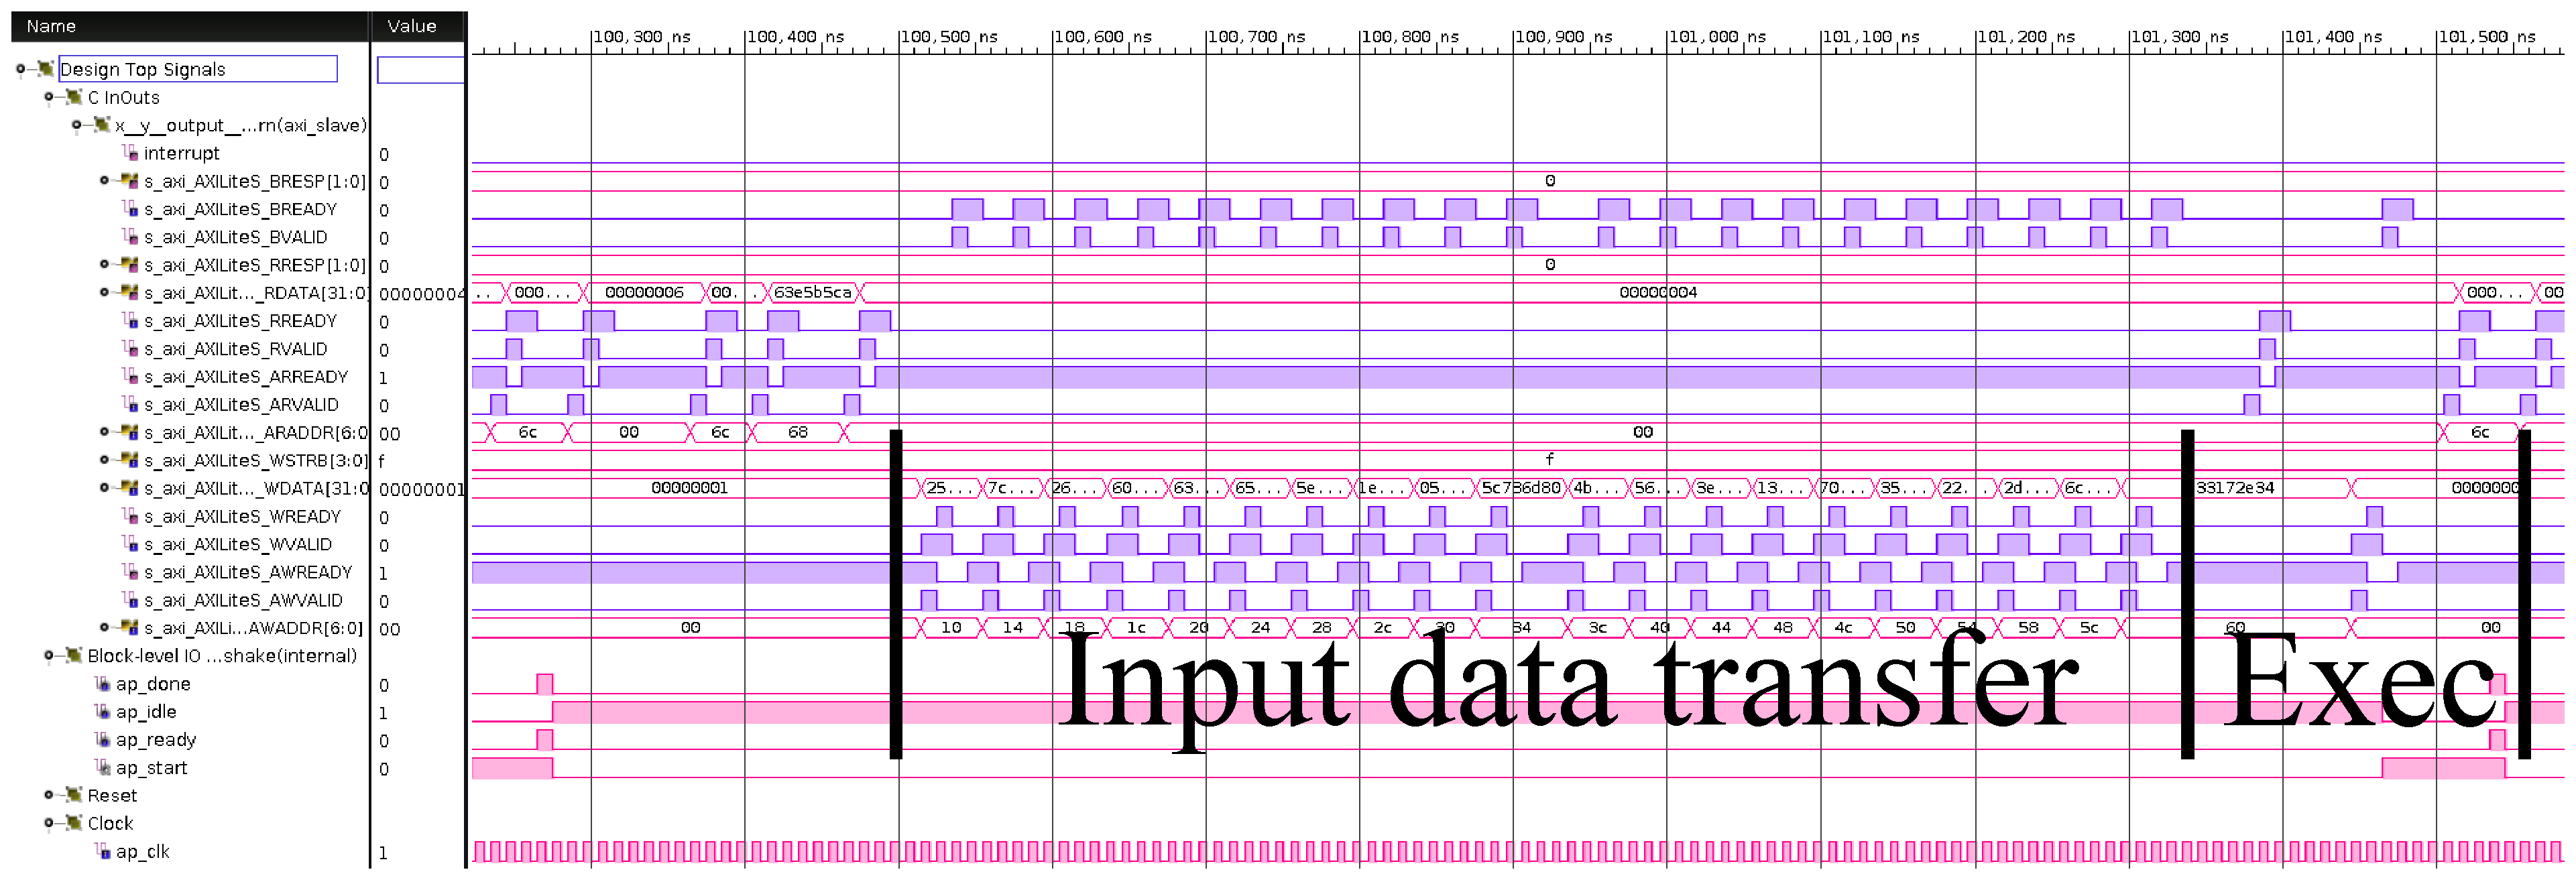
\includegraphics[width=\textwidth]{sim}
	\caption{Simulation waveform. Exec: actual execution time}
	\label{fig:sim}
\end{figure*}



\begin{figure}[!ht]
	\centering
	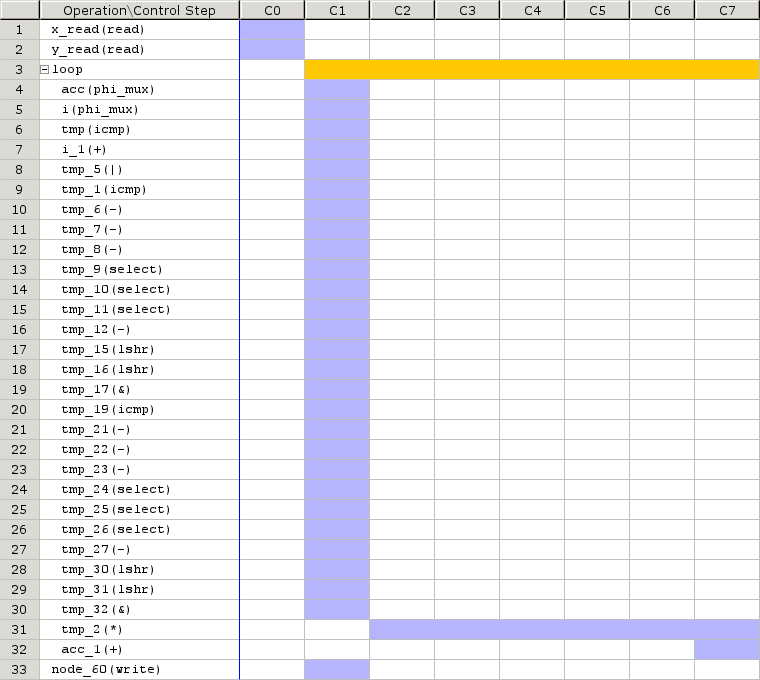
\includegraphics[width=\columnwidth]{none}
	\caption{Performance analysis of unoptimised and pipelined loop}
	\label{fig:none}
\end{figure}


\begin{table}[!ht]
	% increase table row spacing, adjust to taste
	\renewcommand{\arraystretch}{1.3}
	\caption{Resource utilisation of different data width}
	\label{tbl:reswidth}
	\centering
	% Some packages, such as MDW tools, offer better commands for making tables
	% than the plain LaTeX2e tabular which is used here.
	\begin{tabular}{ccccc}
		\hline
		Data width	& BRAM\_18K	& DSP48E	& FF	& LUT	\\
		\hline
		8	& 0	& 10	& 377	& 393	\\
		16	& 0	& 10	& 697	& 745	\\
		32	& 0	& 40	& 990	& 1580	\\
		64	& 0	& 160	& 2250	& 3130	\\
		\hline
	\end{tabular}
\end{table}



\section{Conclusion}

By evaluating the performance data of software and hardware implementation of the same algorithm, the advantages, use case and limiting factors of using hardware accelerators were investigated. Although the computation speed of dedicated hardware accelerator can be faster than software implementation, the data transfer performance may limit the actual efficiency.

The data transfer inefficiency may be improved by using another type of interface, e.g. the AXI4-Stream interface. It transfers data in a sequential streaming manner, would be better than 10 discrete register data transfers.

% references section
%\bibliographystyle{IEEEtran}
%\bibliography{Reference}

% that's all folks
\end{document}
